\chapter{Applicazione realizzata}

\textit{In questo capitolo viene introdotta l'applicazione proposta nell'elaborato in termini di architettura e moduli realizzati ed i passi delle procedure di preparazione e valutazione al fine di ottenere i risultati sperimentali e le relative considerazioni, discusse nei prossimi capitoli. }

\section{Architettura dell'applicazione}
L'applicazione presentata per la comparazione tra software di docking computazionale è organizzata a partire dagli script sviluppati durante il tirocinio interno di circa 300 ore, svolto presso il Consiglio Nazionale delle Ricerche (CNR), alla sede di Napoli.
Sulla base delle analisi proposta per la valutazione dei rischi delle \textit{Apis mellifera} relativamente all'utilizzo dei pesticidi, condotta dal Dott. Ferdinando Febbraio e dalla Dott.ssa Mónica del Águila e seguiti dal Prof. Angelo Ciaramella, è stata realizzata un'applicazione, che fosse in grado di supportare il lavoro di un qualsiasi biologo o biochimico nelle operazioni più classiche di preparazione delle strutture pre-docking, oltre che nell'analisi dei risultati post-docking. Le suddette operazioni, che richiedono un certo livello di \textit{expertize} con i sistemi informativi, sia in termini di manualità sia di ricerca di informazioni, sono spesso procedure meccaniche e macchinose, che rallentano il processo di analisi. Lo sviluppo di tale applicazione ha permesso di automatizzare alcune ma fondamentali operazioni del processo di docking, realizzando un'\textit{Application Program Interface}, più comunemente nota come \textbf{API}, su cui si basa fortemente l'applicazione proposta nell'elaborato. 

L'API è suddivisa in moduli ben distinti che ricoprono le funzionalità dell'applicazione lungo tutta la filiera del docking: dalla fase di preprocessing delle strutture all'analisi delle interazioni dei complessi proteina-ligando. Si è ricorso, quindi, all'utilizzo dei moduli \textbf{MoleculesPreparation} e \textbf{InteractionsAnalysis} per le rispettive fasi di preparazione ed analisi.

I dettagli relativi all'applicazione realizzata durante l'attività di Tirocinio ed ai moduli realizzati saranno definiti esaustivamente nell'elaborato di Tesi triennale in Informatica del collega Alfredo Mungari, prossimo alla laurea nel dicembre 2022, col quale ho condiviso l'intera esperienza di sviluppo.

\section{Scelta del dataset}
A partire dall'esempio di una effettiva applicazione di docking computazionale, presentato precedentemente nella Sezione \ref{Apis mellifera}, la scelta del dataset è ricaduta sulle strutture molecolari tridimensionali della "Apis mellifera" e dei pesticidi coinvolti nella valutazione dei rischi seguita durante il lavoro di tirocinio. Queste strutture indicano rispettivamente l'insieme dei recettori e dei ligandi che saranno utilizzati nel processo di docking, i cui risultati saranno oggetto della comparazione tra i software presentati. 

\subsection{Selezione dei recettori}
Per la selezione dei recettori, si è ricorso al \textbf{Protein Data Bank}, già citato nella Sezione \ref{requirements}. In particolare, la query costruita per recuperare le informazioni dal database considera particolari strutture proteiche che compongono il genoma dell'\textit{Apis mellifera}.

Le api possono essere esposte ai prodotti fitosanitari in due modi: 
\begin{itemize}
    \item per esposizione diretta a \textit{droplets}, che vengono sparse durante l'irrorazione fogliare delle colture, alla polvere della semina durante la semina o all'inalazione di pesticidi volatili durante o dopo l'applicazione alle colture;
    \item dall'esposizione a residui presenti in polline, cera, nettare, miele e gocce di guttazione, che possono derivare dalla contaminazione diretta da spray dei fiori, dalla traslocazione attraverso le piante o dal suolo trattati, o dalla contaminazione diretta durante il trattamento di i favi (solo per le api mellifere);
    \item per esposizione orale ad acqua contaminata \cite{sanchez-bayo_pesticide_2014}.
\end{itemize}

Oltre alle generiche proteine di trasporto, le strutture proteiche selezionate riguardano maggiormente:
\begin{itemize}
    \item le proteine di membrana in quanto alcune di queste sono prese di mira da particolari pesticidi che provocano disturbi alimentari, motori, cognitivi ed infine la morte;
    \item il sistema immunitario per testare le proteine che svolgono un ruolo chiave nell'innescare le risposte immunitarie ai batteri negli insetti;
    \item il sistema olfattivo, anche dette \textit{odorant-binding protein} (OBP), che includono le \textit{pheromone binding protein} (PBP), in quanto sono coinvolte nella rilevazione di odori e feromoni, scaturendo in una segnalazione per attivare un risposta.
\end{itemize}

\begin{figure}
    \centering
    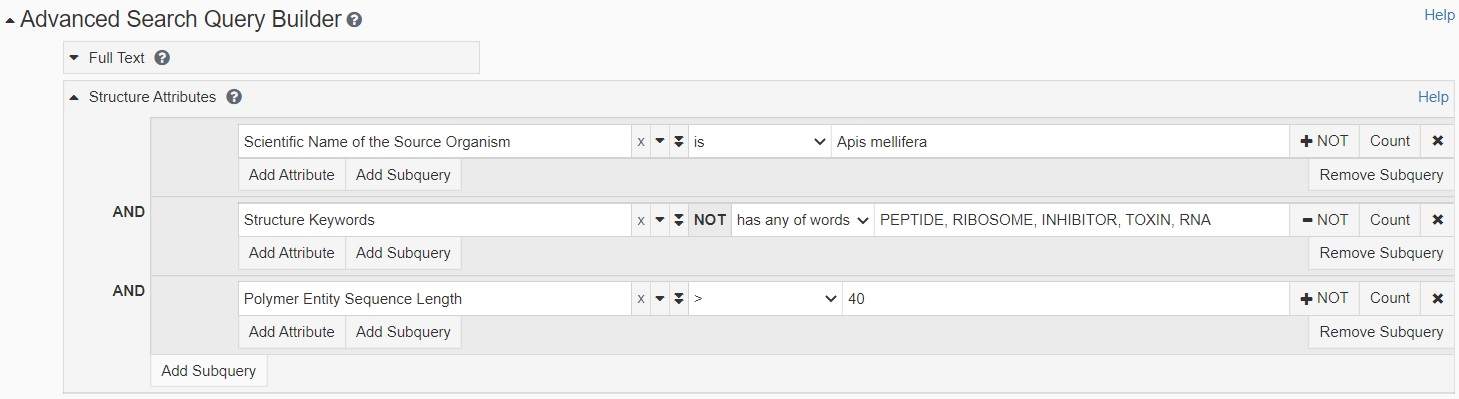
\includegraphics[scale=0.45]{images/chapter3/rcsb_query.jpg}
    \caption[Query per la selezione dei recettori.]{Query per la selezione dei recettori dal sito \url{https://rcsb.org/search/advanced}. La scelta della query e la relativa struttura è illustrata di seguito, nel testo.}
    \label{fig:rcsb_query}
\end{figure}

La selezione delle proteine appena menzionate avviene, quindi, tramite un'interrogazione del Protein Data Bank su attributi come \textit{Scientific Name of the Organism}, \textit{Polymer Entity Sequence Length} per evitare strutture troppo grandi e le \textit{Structure Keywords} che caratterizzano la struttura.

\subsection{Selezione dei ligandi}
Le molecole dei pesticidi sono state selezionate in base all'elenco delle sostanze attive approvate dal database dei pesticidi dell'Unione Europea. Successivamente, le strutture 3D sono state scaricate da \textbf{PubChem} e dall'\textbf{EU Pesticides Database}. 
I pesticidi le cui strutture erano indisponibili in entrambi i database sono stati esclusi dal dataset finale dei ligandi.

La selezione dei ligandi riguarda le strutture dei pesticidi di vario genere come erbicidi, fungicidi e neonicotinoidi, in particolare i piretroidi, a causa della loro nota tossicità.  


\section{Formato dei dati di input ed output}
Le grid-box sono memorizzate nel formato \textit{.txt} mentre le strutture dei recettori e dei ligandi sono fornite rispettivamente nel formato \textit{.pdb} e \textit{.sdf}.
Sia nel caso di recettori sia nel caso di ligandi, al termine della fase di preparazione ed analogamente nella fase di docking, l'output delle strutture è fornito nel formato \textit{.pdbqt}.

\section{Procedura di preparazione al docking} \label{preparation}
Il protocollo di preparazione al docking utilizzato segue dei passi ben definiti per fornire una base equivalente a partire dalla quale effettuare le valutazioni successive alla fase di docking. Tendenzialmente, le fasi di pre-processing delle strutture di input e di post-processing dei risultati del docking sono condivise per entrambi i software, così da non introdurre difformità a monte del processo di valutazione delle prestazioni. 

La fase di pre-processing delle strutture, quindi, consiste nella preparazione dei recettori e dei ligandi.

\begin{table}[H]
\centering
\resizebox{\columnwidth}{!}{%
\begin{tabular}{|cl|}
\hline
\rowcolor[HTML]{9B9B9B} 
\multicolumn{2}{|c|}{\cellcolor[HTML]{9B9B9B}\textbf{Procedura di preparazione}}                                                                                                                                                                                                                                                                                                    \\ \hline
\rowcolor[HTML]{9B9B9B} 
\multicolumn{2}{|c|}{\cellcolor[HTML]{9B9B9B}\textbf{Preparazione delle strutture}}                                                                                                                                                                                                                                                                                                 \\ \hline
\rowcolor[HTML]{C0C0C0} 
\multicolumn{1}{|c|}{\cellcolor[HTML]{C0C0C0}\textbf{Recettori}}                                                                                                                                                                    & \multicolumn{1}{c|}{\cellcolor[HTML]{C0C0C0}\textbf{Ligandi}}                                                                                 \\ \hline
\multicolumn{1}{|l|}{\begin{tabular}[c]{@{}l@{}}• separazione dei residui ripetuti\\ • epurazione da catene di eteroatomi\\ • rimozione di catene duplicate\\ • applicazione di prepare\_receptor4.py \\ (modificato)\end{tabular}} & \begin{tabular}[c]{@{}l@{}}• conversione da .sdf a .pdb\\ • conversione da .pdb a .pdbqt\\ • applicazione di prepare\_ligand4.py\end{tabular} \\ \hline
\end{tabular}%
}
\caption[Riepilogo delle procedura di preparazione.]{Riepilogo delle procedura di preparazione. A sinistra la procedura di preparazione dei recettori, a destra la procedura di preparazione dei ligandi. }
\label{preparation_table}
\end{table}

Per i due software, il concetto di \textit{best binding pose} è notevolmente diverso. 
Il software AutoDock Vina considera la migliore posa tra tutte quelle possibili nello spazio conformazionale di ricerca quella che risulta avere l'\textit{affinità} minore. A parità di affinità, viene selezionata la posa la cui RMSD\footnote{In bioinformatica, la Root Mean Square Deviation delle posizioni atomiche è la misura della distanza media tra gli atomi di proteine sovrapposte.} risulta essere minore.

Nel caso del sofware GNINA, il criterio utilizzato è quello predefinito CNNscore, introdotto nella Sezione \ref{cnn_params}. Tuttavia, nulla vieta di fissare un criterio differente in base al tipo di analisi che si vuole effettuare.


\subsection{Preparazione dei recettori}
Nel caso specifico, la preparazione dei recettori richiede alcune operazioni direttamente implementate ed altre solitamente applicate nella fase di preparazione.

Le operazioni direttamente implementate riguardano la separazione di residui ripetuti, l'epurazione da catene di eteroatomi e la rimozione di catene molecolari duplicate.

La \textbf{separazione dei residui ripetuti} riguarda quelle ripetizioni dei residui nelle catene molecolari della struttura del recettore. Quest'informazione è comunemente nota come \textit{"alternative location"} e codificata come \textit{alt\_loc}. La \textbf{pulizia di catene di eteroatomi} consiste nell'epurazione della struttura da catene formate esclusivamente da eteroatomi, non interessanti per il processo di docking. Successivamente viene eseguita la \textbf{rimozione delle catene molecolari duplicate} e considerate solo catene distinte tra le catene molecolari presenti all'interno della struttura.

Inoltre, la preparazione include la rimozione delle molecole d'acqua e di eventuali ligandi non standard residui, l'aggiunta di atomi di idrogeno polari e cariche di Kollman e l'unione delle cariche e la rimozione di atomi di idrogeno non polari e delle coppie molecolari slegate. Infine, sono state create le \textit{grid-box} con una spaziatura di 3Å (angstroms) per scansionare la superficie della proteina.
Per effettuare queste operazioni, è stato applicato uno script modificato di \textbf{prepare\_receptor4.py} prodotto dallo Scripps Research Institute, distribuito nelle suite MGLTools ed AutoDockFR e comunemente utilizzato nelle fasi di pre-processing dei recettori. Tale modifica consiste nella possibilità di aggiungere cariche di Kollman, piuttosto che esclusivamente cariche di Gasteiger, risultando in un'estensione dello script. 


\subsection{Preparazione dei ligandi}
Relativamente alle strutture dei ligandi, non vengono effettuate particolari operazioni se non la conversione di formato e operazioni svolte comunemente nella preparazione classica dei ligandi. 
A tal proposito, è stato utilizzato \textbf{OpenBabel} per la conversione del formato della struttura e successivamente lo script \textbf{prepare\_ligand4.py}, prodotto dallo Scripps Research Institute, distribuito nelle suite MGLTools ed AutoDockFR.
La preparazione include l'unione delle cariche e la rimozione di atomi di idrogeno non polari e delle coppie molecolari slegate.


\subsection{Fase di docking}
Per i due software in competizione, è mostrato il commando lanciato con i relativi parametri. Per ogni parametro è fornita una breve descrizione.

Di seguito è riportato il comando lanciato per effettuare il docking utilizzando AutoDock Vina e la relativa tabella esplicativa dei parametri.


\begin{minted}[breaklines]{bash}
  $ vina --config <text_file> --receptor <receptor_file> --ligand <ligand_file> --out <output_file> --log <text_file>
\end{minted}
%

\begin{table}[H]
\centering
\resizebox{\columnwidth}{!}{%
\begin{tabular}{|c|l|}
\hline
\rowcolor[HTML]{C0C0C0} 
\multicolumn{1}{|l|}{\cellcolor[HTML]{C0C0C0}\textbf{Parametro}} & \textbf{Descrizione del parametro}                                                                                                                                                                         \\ \hline
\textit{--config}                                                         & \begin{tabular}[c]{@{}l@{}}Consente di allegare un file di configurazione, il quale contiene\\ le informazioni come l'\textit{exhaustiveness} e i parametri della grid-box,\\ come file di testo (txt)\end{tabular} \\ \hline
\textit{--receptor}                                                       & Seleziona il recettore per cui effettuare il docking                                                                                                                                                       \\ \hline
\textit{--ligand}                                                         & Seleziona il ligando per cui effettuare il docking                                                                                                                                                         \\ \hline
\textit{--out}                                                            & Consente di esportare la pose con il valore di affinità maggiore                                                                                                                                           \\ \hline
\textit{--log}                                                            & \begin{tabular}[c]{@{}l@{}}Permette di salvare un file di logging contenente le informazioni\\ dall'avvio del comando fino al termine del docking, come file di\\ testo (txt).\end{tabular}                \\ \hline
\end{tabular}%
}
\caption[Tabella dei parametri per il docking con AutoDock Vina.]{Tabella dei parametri del comando per il docking utilizzando AutoDock Vina. A sinistra sono illustrati i paramentri, a destra la relativa descrizione.}
\end{table}

Di seguito è riportata il comando lanciato per effettuare il docking utilizzando GNINA e la relativa tabella esplicativa dei parametri. Per questioni di chiarezza, sono riportati anche i parametri impliciti e predefiniti della commandline.

\begin{minted}[breaklines]{bash}
  $ gnina --receptor <receptor_file> --ligand <ligand_file> --autobox_ligand <receptor_file> --cnn_verbose
\end{minted}

\begin{table}[H]
\centering
\resizebox{\columnwidth}{!}{%
\begin{tabular}{|c|l|}
\hline
\rowcolor[HTML]{C0C0C0} 
\textbf{Parametro}           & \textbf{Descrizione del parametro}                                                                                                                      \\ \hline
\textit{--receptor}          & Seleziona il recettore per cui effettuare il docking                                                                                                    \\ \hline
\textit{--ligand}            & Seleziona il ligando per cui effettuare il docking                                                                                                      \\ \hline
\textit{--autobox\_ligand}   & \begin{tabular}[c]{@{}l@{}}Permette di indicare la struttura del recettore contenente il ligando\\ naturale, qualora questo fosse presente\end{tabular} \\ \hline
\textit{--scoring}           & \begin{tabular}[c]{@{}l@{}}Permette di selezionare la funzione di scoring da utilizzare inizialmente \\ (Vina, predefinito)\end{tabular}                                                                            \\ \hline
\textit{--cnn\_scoring}      & \begin{tabular}[c]{@{}l@{}}Consente di specificare in quale fase del processo di docking utilizzare\\ la funzione di scoring CNN (rescore, predefinito)\end{tabular}           \\ \hline
\textit{--pose\_sort\_order} & \begin{tabular}[c]{@{}l@{}}Permette di selezionare il criterio secondo il quale effettuare il ranking\\ delle pose (CNNscore, predefinito)\end{tabular}                         \\ \hline
\textit{--cnn\_verbose}      & \begin{tabular}[c]{@{}l@{}}Maggiori informazioni sono messe a schermo aumentando la \\ verbosità del software\end{tabular}                              \\ \hline
\end{tabular}%
}
\caption[Tabella dei parametri per il docking con GNINA.]{Tabella dei parametri interessanti, impliciti ed espliciti del comando per il docking utilizzando GNINA. A sinistra sono illustrati i paramentri, a destra la relativa descrizione.}
\end{table}

\section{Procedura di valutazione delle prestazioni} \label{evalutation}
La fase di post-processing, introdotta nella Figura \ref{evaluation_table}, consiste nell'utilizzo di metriche per valutare le prestazioni del docking, in primo luogo della rete neurale convoluzionale applicata nel software GNINA, e successivamente del software AutoDock Vina, che analizzano diversi aspetti del risultato di un esperimento di \textbf{single blind docking}: dalla visualizzazione delle pose predette al criterio di distanza tra il recettore e la migliore pose del ligando alla rilevazione ed analisi delle interazioni molecolari osservate nel complesso, sia in termini qualitativi e quantitativi, sintetizzate attraverso \textit{heatmap} e istogramma, sia in termini di valori medi dei parametri di output dei software corrispondenti.


\begin{table}[H]
\centering
\resizebox{\columnwidth}{!}{%
\begin{tabular}{|cll|}
\hline
\rowcolor[HTML]{9B9B9B} 
\multicolumn{3}{|c|}{\cellcolor[HTML]{9B9B9B}\textbf{Procedura di valutazione}}                                                                                                                                                                                                                                                                                                                                                                                                                                                                                                                                                                                                 \\ \hline
\rowcolor[HTML]{9B9B9B} 
\multicolumn{3}{|c|}{\cellcolor[HTML]{9B9B9B}\textbf{Analisi delle interazioni}}                                                                                                                                                                                                                                                                                                                                                                                                                                                                                                                                                                                                \\ \hline
\rowcolor[HTML]{C0C0C0} 
\multicolumn{1}{|c|}{\cellcolor[HTML]{C0C0C0}\textbf{Rilevazione}}                                                           & \multicolumn{1}{c|}{\cellcolor[HTML]{C0C0C0}\textbf{Analisi}}                                                                                                                                                                                                                                   & \multicolumn{1}{c|}{\cellcolor[HTML]{C0C0C0}\textbf{Visualizzazione}}                                                                                                                                                                          \\ \hline
\multicolumn{1}{|l|}{\begin{tabular}[c]{@{}l@{}}• rilevazione di legami (close \\ contacts, legami a idrogeno)\end{tabular}} & \multicolumn{1}{l|}{\begin{tabular}[c]{@{}l@{}}• calcolo della MSC RMSD\\ • calcolo delle medie per \\i parametri di output (CNNscore,\\ CNNaffinity, affinity)\\ • calcolo della magnitudo della \\ differenza tra le medie per il \\ parametro affinity\\ • tempi del docking\end{tabular}} & \begin{tabular}[c]{@{}l@{}}• rimozione di remarks\\non necessari \\ • visualizzazione delle pose\\ predette\\ • visualizzazione delle\\ interazioni attraverso\\ heatmap\\ • visualizzazione delle\\ interazioni attraverso\\ istogramma\end{tabular} \\ \hline
\end{tabular}%
}
\caption[Riepilogo della procedura di valutazione.]{Riepilogo della procedura di valutazione delle prestazioni. A sinistra la fase di rilevazione dei legami, al centro le fasi percorse per l'analisi delle interazioni, a destra le operazioni per la visualizzazione delle interazioni. }
\label{evaluation_table}
\end{table}

Onde evitare problematiche nell'apertura dei file dei ligandi prodotti con GNINA per la visualizzazione in AutoDockTools, i file di output, in formato .pdbqt, sono modificati rimuovendo linee di testo non necessarie ai fini della visualizzazione.

\subsection{Rilevazione delle interazioni}
A partire dalla possibilità di mostrare le interazioni tra un recettore ed un ligando fornita da AutoDockTools, è stato sviluppato uno script che permettesse di ottenere e memorizzare tali informazioni per ulteriori scopi ed analisi.

Per tal motivo, è stata eseguita un'ispezione approfondita del codice sorgente di AutoDockTools, scritto in Python2, riuscendo così ad estrarre tale funzionalità. L'informazione relativa alle interazioni è memorizzata nella classe \textit{InteractionDescriptor}. Sfruttando quest'informazione, relativa alla classe ed ai metodi implementati, è stato possibile ricavare il numero di \textbf{close contact} e \textbf{legami a idrogeno}, importanti per valutare la stabilità e la forza del legame.

Un legame a idrogeno è un particolare legame che si forma tra un atomo di idrogeno legato covalentemente a un atomo fortemente elettronegativo (detto donatore) e un secondo atomo anch’esso elettronegativo (detto accettore). 

Nel conteggio dei legami a idrogeno vengono considerati quei legami in cui atomi di un certo residuo proteico risultano essere accettori o donatori.

\subsection{Minimized Symmetric-Corrected RMSD} \label{mscrmsd}
Per valutare la bontà delle predizioni effettuate da GNINA, uno dei criteri è la Root Mean Square Deviation o meglio nota come RMSD. Tuttavia, non è stata adoperata la classica RMSD, bensì quella con la correzione della simmetria, anche nota come Symmetric-Corrected RMSD, che considera la simmetria della molecola nel calcolo della RMSD, successivamente minimizzata, che prende il nome di \textbf{Minimized Symmetric-Corrected RMSD}.

I dati riportati sono stati ottenuti utilizzando la libreria \textbf{spyrmsd}, che permette di calcolare la MSC RMSD. 

Ai fini di un'analisi di valutazione dei rischi, questo passaggio non è granchè significativo, in quanto le strutture sono cristallizzate e rigide; tuttavia, viene considerato per osservare l'accuratezza della predizione dei software rispetto alle caratteristiche di tali strutture.
\subsection{Visualizzazione delle interazioni} \label{charts}
Le interazioni osservate dopo la fase di rilevazione sono sintetizzate in due tipi di grafici che hanno due scopi differenti.

Un \textit{heatmap} è una rappresentazione grafica dei dati dove i singoli valori contenuti in una matrice sono rappresentati da colori. Nel nostro caso, i dati visualizzati riguardano il tipo di legame formato tra il residuo di una proteina ed il ligando. 

I possibili legami possono appartenere a tre tipi di categorie o contatti differenti: nessun legame, legame a idrogeno e "close contact", in cui semplicemente atomi di recettore e ligando sono sufficientemente vicini ma non formano alcun legame chimico. 
Questa tipo di rappresentazione possiamo definirla \textit{ligand-oriented} in quanto ci consente di raggruppare visivamente ligandi che producono la maggior parte delle interazioni.


Un istogramma è un diagramma che fornisce una rappresentazione di un insieme di dati mediante un grafico a barre. L'istogramma realizzato mostra i residui coinvolti nelle interazioni proteina-ligando, il numero di interazioni di tipo "close contact" e legami a idrogeno e la lista di ligandi con cui si verificano questi contatti.
A differenza dell'heatmap, questo tipo di rappresentazione possiamo definirla \textit{protein-oriented} in quanto mette in evidenza i residui coinvolti nella maggior parte delle interazioni, identificati attraverso i picchi dell'istogramma.



